\documentclass[11pt, 
]{IEEEtran}
\usepackage{cite}
\usepackage{moreverb}
\usepackage{amsfonts}
\usepackage[pdftex]{graphicx}
\usepackage{comment}
\usepackage{enumitem}
\usepackage{array}

\newtheorem{theorem}{Theorem}

\newcommand{\specialcell}[2][c]{\begin{tabular}[#1]{@{}c@{}}#2\end{tabular}}

\hyphenation{op-tical net-works semi-conduc-tor}

\begin{document}

\title{The Impact of Immersive Exergaming in Virtual Reality}

% author names and affiliations
% use a multiple column layout for up to two different
% affiliations
\author{\IEEEauthorblockN{Jonathan Curtin, Timothy Diack, Christopher Morgan, Christopher Pearce}\\
\IEEEauthorblockA{
Department of Computer Science\\
The University of Auckland\\
38 Princes Street, Auckland 1020, New Zealand\\
Email:~{\tt \{jcur884, tdia010, cmor149, cpea144\}@aucklanduni.ac.nz}
}}

\maketitle

\begin{abstract}

Previous studies show that exergaming has a positive impact on user’s motivation to exercise over traditional methods. Unfortunately, these studies also show a lack of adherence over a longer term. This project aims to study the effects of virtual reality while playing an exergame and whether the immersion provided has a positive impact on the chances of continued use. We believe that the immersive atmosphere of the virtual reality is of secondary importance to the immersion of the game itself in terms of causing user adherence. The exergame is played with an exercise bike, with the Oculus Rift used to provide the virtual reality simulation.

The proposed game was evaluated with a user study which compared the game using an Oculus Rift, the game using a typical screen, and the exercise by itself with no game. We found that the use of a game both with and without the Oculus Rift scored much higher than the exercise alone. Another thing to note is that the scores of the game with and without the Oculus Rift scored very similarly to each other, with the Oculus only scoring slightly higher. We attribute this to the extra immersion of virtual reality.
 
\end{abstract}

\begin{IEEEkeywords}
Virtual reality, exercise, video game, motivation
\end{IEEEkeywords}


\section{Introduction} \label{Introduction}

Exercising frequently is well known to provide many benefits to a person's general health, such as boosting their immune system, preventing heart disease, diabetes, and obesity. It has also been shown to help prevent depression, promote self-esteem, and improve a person's mental health. With the growing concern of childhood obesity, motivating people to exercise has become a valuable and important task.

One approach to this problem that is of particular interest to us is the combination of exercise and gaming (known as exergaming). Many studies have shown that exergames are good enough to meet general exercise requirements; however they do not necessarily provide the motivation to continue with the program over longer periods of time. This is partially as the main focus of these studies has been to prove that exergaming contains an adequate amount of exercise to obtain the benefits listed above. Very few studies have focused on the motivation to play these games repeatedly, thus resulting in a lack of adherence by the users.

Motivation is a key element towards people wanting to continue with the exercise program. In this paper, we present a study focusing on whether competition between different players is more motivating than attempting to beat a high score in an exergame. In particular, we wish to answer the question: How does competition against another person affect the motivation to continue exercising?

%If the addition of cognitive tasks improve motivation

For this project we have created an exergame in which the player uses the exercycle to power a helicopter-esque vehicle to retrieve a series of targets from different locations in the world. We utilize both the exercycle (to provide the ability to move up and down) and the Oculus Rift (to add steering capabilities based on where the player is looking).

To answer our research question, we performed a user study comparing three different scenarios in the exergame we created. The first was just competing against a high score based on how long it took to finish the course. The second scenario was competing against a 'ghost' of the player's past performance. The final scenario was competing against a different player's past performance.

The rest of the paper is split into the following sections: section II contains a list of related papers on exergaming studies on motivation; section III explains the design decisions for the exergame; section IV details the implementation of our game and how it functions; section V shows our results and evaluations; finally section VI is a conclusion of our findings and contributions.

\section{Related Works} \label{Related Works}

Caldwell et al. \cite{caldwell2013intersection} performed a case study on the ability for video games to help provide patient empowerment via positive metaphoric visualization. While the experiment was originally inspired by a child battling cancer, the concept of empowerment could be applied to many different aspects of life such as exercising. It is stated that engagement is a significant factor in the success of their experiments. This approach relates to our work in that we have asked our participants to compare the different approaches to keeping them engaged and increasing user adherence.

Reeve \cite{reeve1996elements} explored the elements of competitiveness that affect intrinsic motivation. Intrinsic motivation is derived from a need for self-determination and competence. Reeve tested aspects such as competition between participants against beating personal bests, and their effect on the participant's motivation. While the results of his study showed that the elements of competitive outcome and interpersonal context do affect intrinsic motivation, past studies have been inconclusive due to the different circumstances and types of competition. Due to this information, our study focused on whether or not these aspects have an effect on exergaming adherence.

Song et al. \cite{song2010effects} investigated the effects of competition on intrinsic motivation in exergaming and the side-effects of presence. They tested a 2 by 2 design of experiment: Competition against Non-competition, and High individual competitiveness against Low. This study has many similarities with our own study, although we have kept our focus on the differences between competing for a high score versus competing against the participant's past performance versus competing against a different participant's past performance. Also, due to the nature of our exergame being in virtual reality, we could discover if the added immersion had any positive or negative effects.

Mokka et al. \cite{mokka2003fitness} developed a fitness game for a virtual fitness centre aimed at increasing the motivation and richness of the experience. Unfortunately, they had issues with the participants focusing on the exercise rather than the game itself. This has similarities to our project in that we used virtual reality to create the world for the participants. However, with the help of the Oculus Rift, users had added immersion which helped to keep the focus on the game instead of the fact that they were exercising.

\section{Design} \label{Design}

In response to our research question, we chose to design an exergame that would be detached from the realities of the exercise in question (in our case, cycling). As we would like to ascertain the effects of cognitive stimulation on motivation, the exergame would incorporate cognitive tasks to help simulate both the brain and body simultaneously. We created two versions of a race course, one with simple point scoring mechanics, and the other containing simple cognitive tasks for the users to complete. 

Although studies on competitiveness, such as \cite{reeve1996elements} and \cite{song2010effects} have been performed in the past, none of them have focused on whether cognitive tasks affect people's motivation, and therefore this was the contribution that we wish to add.

\subsection{Exergame}

This decision to detach the exergame from the specific exercise was made in light of studies such as \cite{caldwell2013intersection} which describes engagement as being a large factor on the success of projects like this and \cite{mokka2003fitness} in which the participants had issues focusing on the game over the exercise itself. Unfortunately, this brought a separate problem of choosing a task that still intuitively made sense to the participants. 

In our case, we chose a helicopter and related the exercise of cycling to the rotations of the helicopter's blades. While there were many vehicles that could perform similarly, we decided that linking the speed of the person peddling to how fast the rotor blades were spinning provided an interaction that was clear to all the people using it i.e. peddling fast results in the helicopter ascending, while not peddling will result in rapid descent.

\subsection{Cognitive tasks}

Choosing a way to cognitively engage the users was a difficult obstacle in our design process. Due to the wide array of tasks to choose from, there is a high possibility of many effective ways to do this. Ideas such as pattern recognition, moving objects, and answering simple questions were considered by our group and we ultimately settled on answering questions. 

Pattern recognition has a tendency to either be too simple or overly difficult and abstract. We avoided choosing to move objects around, despite prototyping a tractor beam for the helicopter, due to our desire for the race course to have a flow to it. This meant we did not wish the players to have to stop and collect objects as we felt this would break the rhythm and forward progression. 

We eventually decided on answering simple questions as this provided the advantage of being easily changed to various topics if the creators needed. By making the questions multiple choice we could also easily provide methods in the world to answer them such as sets of rings which have the different potential answers in them.

\begin{figure}[tb]
	\centering
		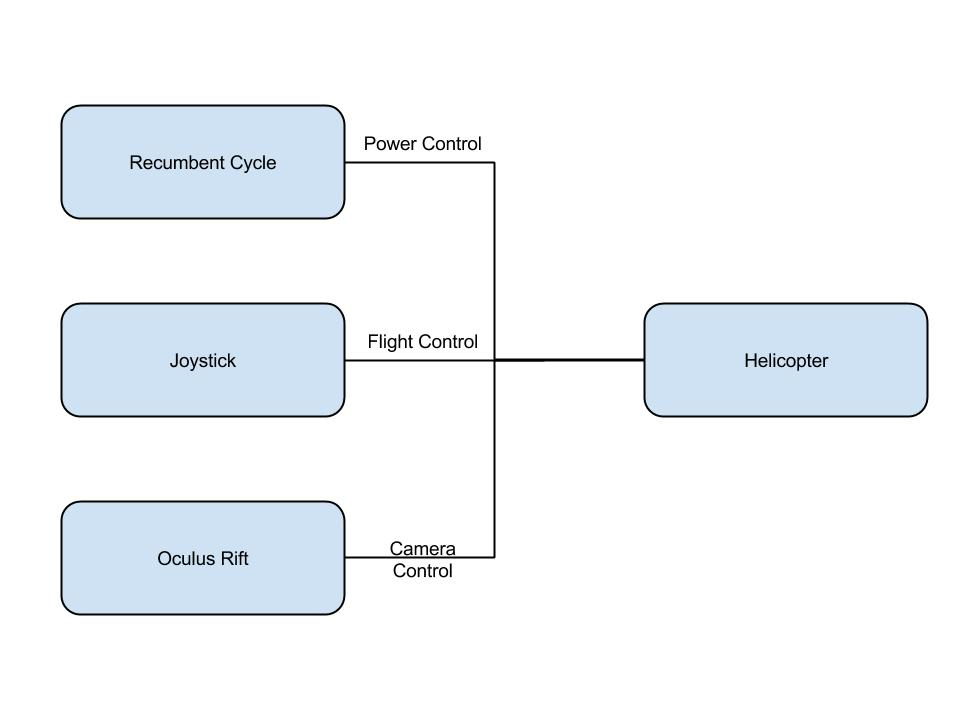
\includegraphics[width=1\columnwidth]{Diagram.jpg}
	\caption{Interactions of the hardware and our helicopter}
	\label{fig:helicopter}
\end{figure}

\section{Implementation} \label{Implementation}

The prototype exergame we created has been implemented in the Unity game engine. Obviously the biggest challenge for creating an entire exergame from nothing is the amount of content required (such as models, courses to race on, cognitive tasks, etc), as well as the time frame in which to create all of it. In order to make this task manageable, we have chosen to only create one course for our prototype.

To create some of the models used in our project (such as the helicopter itself) we have used Blender. The .blend files are then imported as assets which Unity automatically converts into .fbx files to be attached to game objects.

Another challenge that we had to overcome was the way in which we provide simple cognitive tasks for the users. While this went through several iterations, we ultimately chose to convey some simple questions through the screen in the cockpit of the helicopter. The answers would then be given as a set of rings in the world of which you could only go through one per question. Correct answers would be rewarded with a temporary speed boost as well as a lowering of the resistance on the cycle itself, while incorrect answers would increase the resistance temporarily.

The other hardware involved in this project include a Logitech Extreme 3d Pro Joystick, the Oculus Rift DK1, and an exercycle provided by the university. The joystick provides the users a more intuitive and natural way of controlling the helicopter's tilt, pitch, yaw, and movement. The Oculus Rift enables the user's ability to look around freely without the need to move. And finally the exercycle allows the user to control the rotors of the helicopter, and therefore the up and down movement. It is clearly also the type of exercise we have chosen for our exergame. The exercycle interfaces with Unity via a C\# script provided by Lindsay Shaw, while the Oculus SDK already has integration with Unity.

\section{Evaluation}

\subsection{Methodology}

We have investigated how an exergame utilizing simple cognitive tasks would affect the motivation of users. To achieve this we created two versions of a single main course. The first version is time-trial based, with the users receiving points for how many checkpoints they pass. The second version contains coloured rings at each checkpoint, and a simple memory game is played via floating coloured orbs inside the cockpit of the helicopter. This game involves memorizing the order of colours and then passing through the correct coloured ring at each checkpoint. Each time the sequence is completed, the length of the sequence is increased by one and the new sequence is briefly shown to the user.

The participants were given approximately 2-5 minutes each to familiarize themselves with the controls, and then they were given 6 minutes to get as far as they could with each version of the main course. To reduce learning bias as much as possible, half of the participants started on the first version and half on the second.
Users were also asked to fill out several questionnaires during the experiment. Table \ref{table:preq} shows us the questions they filled out before the experiment, table \ref{table:interq} was filled out after each of the two tasks (once per task), and table \ref{table:postq} was filled out at the end of the experiment.

The experiments were carried out over two days, taking approximately 30 minutes per participant. Since each of these days were managed by different members of our team, a script was created and used to keep testing conditions as standard as possible, and reduce the amount of bias between sessions. Important aspects of the experiments such as how much help should be given to participants and what order tasks should be performed were described in this script.

We also wanted to measure the user's heart rates using a simple heart rate monitor on a watch to find out if the exergame provides sufficient exercise to benefit potential future clients. This also would allow us to discover if the two differing versions of the game provide different amounts of physical stress for users. Unfortunately, this did not eventuate and the consequences will be discussed later.

\subsection{Results} %up to date

We performed this experiment with 10 participants, and recorded the non-short answer questions in tables \ref{table:preres}, \ref{table:nonres}, \ref{table:cogres}, and \ref{table:postres}.

When asked whether the memorization task had any effect on their performance versus not having to memorize anything, participants were divided. While there were a range of answers, such as the extra task improving performance since they were more focused on memorizing the sequence or that it took their mind off the actual pedalling, the majority were closely split between two main answers. Three participants thought that the extra task made little to no difference to their performance, and four participants believed that it made the experiment slightly more difficult.

The next question asked which mode would be preferred to be used as a form of entertainment, to which participants had a clear favourite: six people stated that they would prefer the version with the cognitive task as a form of entertainment. The remainder of the participants were evenly divided between the non-cognitive version, both versions being equal, and neither version being preferable.

Similar to the second question, participants were then asked which mode would be preferred to be used as a form of exercise. Once again, six people chose the cognitive version, but unlike the previous question, all of the remaining people chose the non-cognitive version as their preferred option.

The final question asking for comments and suggestions received a large range of answers. Some comments asked for improvements to the current build such as improving the control scheme, changing the visuals of the helicopter to look more like helicopters in real life, adding methods for colour-blind people to tell the rings apart, and the ability to change the difficulty to help get used to the controls. Others contained suggestions to include guns and/or multiplayer, or just commented that it was an enjoyable experience.

\subsection{Discussion}

A total of 10 people volunteered for this experiment (8 men and 2 women), all between the ages of 18-24. 9 out of ten identified themselves as students, with the 10th having marketing as an occupation. The students came from several different faculties in the university. While this could be a potential threat to validity due to self-selection bias, it can also be useful since 20.6\% of adults aged 15-24 in New Zealand are considered obese. This statistic continues to rise as we look at older demographics; therefore targeting this age group is an important step in prevention of obesity in older age groups.

One major threat to validity was the lack of a heartbeat monitor during the experiments. By not measuring the exertion of our participants, we have no way of determining if our exergame provides sufficient exercise. This also renders our question about perceived exertion relatively useless as we cannot compare the answers with empirical evidence. Despite this, an interesting statistic to note is that on average, the participants believed that the non-cognitive mode required more exertion that the cognitive mode. This could be due to focusing more on the memorization task, thus taking their minds off the exercise itself.

Another interesting statistic is while 6 people found the cognitive exergame more motivating, the answer to whether they prefer the exergame to traditional exercise was much more divided with 3 disagreeing, 4 people agreeing, and the remainder staying neutral. This could be due to a variety of reasons, but unfortunately we did not have a follow-up question to find out.

Many of the other threats to validity such as order bias, training effect, fatigue, misunderstandings, and social desirability were all taken into consideration to minimize their effects on the experiment.

\begin{table*}
    \begin{center}
        \begin{tabular}{|p{5cm}|c c c c c|}
        \hline
		Age: &12-17 &18-24 &25-34 &35-44 &45+\\
		\hline
		Gender: & & Male & & Female & \\
		\hline
		Occupation: & & & & & \\
		\hline
		\hline
		& Daily & \specialcell{Two-Three\\times a week} & Weekly & Monthly & Never \\
		\hline
		Have you used an Oculus Rift/VR headset before? & 1 & 2 & 3 & 4 & 5 \\
		\hline
        Have you used a joystick before? & 1 & 2 & 3 & 4 & 5 \\
		\hline
		Have you used an exercycle/bicycle before? & 1 & 2 & 3 & 4 & 5 \\
		\hline
		How often do you exercise? & 1 & 2 & 3 & 4 & 5 \\
		\hline
		How often do you play video games? & 1 & 2 & 3 & 4 & 5 \\
		\hline
		\hline
		& \specialcell{Strongly\\Disagree} & Disagree & Neutral & Agree & \specialcell{Strongly\\Agree} \\
		\hline
		I consider myself physically fit & 1 & 2 & 3 & 4 & 5 \\
		\hline
		I feel physically fit today. & 1 & 2 & 3 & 4 & 5 \\
		\hline
		I enjoy exercising. & 1 & 2 & 3 & 4 & 5 \\
		\hline
		I enjoy playing video games. & 1 & 2 & 3 & 4 & 5 \\
		\hline
        \end{tabular}
    \end{center}
    \caption{Pre-Questionnaire}
    \label{table:preq}

    \begin{center}
        \begin{tabular}{|p{5cm}|c c c c c|}
        \hline
        & \specialcell{Strongly\\Disagree} & Disagree & Neutral & Agree & \specialcell{Strongly\\Agree} \\
        \hline
        I found the experience physically challenging.& 1 & 2 & 3 & 4 & 5 \\
        \hline
        I felt comfortable while using the system.& 1 & 2 & 3 & 4 & 5 \\
        \hline
        I experienced motion sickness while playing the game.& 1 & 2 & 3 & 4 & 5 \\
        \hline
        I felt physically challenged while using the system.& 1 & 2 & 3 & 4 & 5 \\
        \hline
        I felt cognitively challenged while using the system.& 1 & 2 & 3 & 4 & 5 \\
        \hline
        Playing the exergame was enjoyable overall.& 1 & 2 & 3 & 4 & 5 \\
        \hline
        The exergame was immersive.& 1 & 2 & 3 & 4 & 5 \\
        \hline
        On a scale of 6-20, what number best describes your level of exertion? & & & & & \\
        \hline
        \end{tabular}
    \end{center}
    \caption{Post-Task Questionnaire}
    \label{table:interq}

    \begin{center}
        \begin{tabular}{|p{5cm}|c c c c c|}
         \hline
         & \specialcell{Strongly\\Disagree} & Disagree & Neutral & Agree & \specialcell{Strongly\\Agree} \\
		\hline
		I enjoyed playing the exergame. & 1 & 2 & 3 & 4 & 5 \\
		\hline
		I would prefer to exercise using this exergame rather than through traditional means. & 1 & 2 & 3 & 4 & 5 \\
		\hline
		I found the game with the cognitive exercises more motivating. & 1 & 2 & 3 & 4 & 5 \\
		\hline
		How do you think the additional task affected your performance? & & & & & \\
		\hline
		Which of the modes of play would you prefer to use as a form of entertainment? & & & & & \\
		\hline
		Which of the modes of play would you prefer to use as a form of exercise? & & & & & \\
		\hline
		Comments and Suggestions? & & & & & \\
		\hline
        \end{tabular}
    \end{center}
    \caption{Post-Questionnaire}
    \label{table:postq}
\end{table*}








\begin{table*}
    \begin{center}
        \begin{tabular}{|p{5cm}|c c c c c|}
        \hline
		Age: & 18-24 & & & & \\
		\hline
		Gender: & & Male: 8 & & Female: 2 & \\
		\hline
		Occupation: & & Student: 9 & & Marketing: 1 & \\
		\hline
		\hline
		& Daily & \specialcell{Two-Three\\times a week} & Weekly & Monthly & Never \\
		\hline
		Have you used an Oculus Rift/VR headset before? &  &  &  & 1 & 9 \\
		\hline
        Have you used a joystick before? &  &  &  & 1 & 9 \\
		\hline
		Have you used an exercycle/bicycle before? & 1 & 1 &  & 3 & 5 \\
		\hline
		How often do you exercise? & 3 & 2 & 4 &  & 1 \\
		\hline
		How often do you play video games? & 3 & 3 & 1 & 3 &  \\
		\hline
		\hline
		& \specialcell{Strongly\\Disagree} & Disagree & Neutral & Agree & \specialcell{Strongly\\Agree} \\
		\hline
		I consider myself physically fit &  & 1 & 2 & 4 & 3 \\
		\hline
		I feel physically fit today. & 1 &  & 4 & 4 & 1 \\
		\hline
		I enjoy exercising. & 1 &  & 2 & 6 & 1 \\
		\hline
		I enjoy playing video games. &  &  &  & 4 & 6 \\
		\hline
        \end{tabular}
    \end{center}
    \caption{Pre-Questionnaire Results}
    \label{table:preres}
\end{table*}

\begin{table*}
    \begin{center}
        \begin{tabular}{|p{5cm}|c c c c c|}
        \hline
        & \specialcell{Strongly\\Disagree} & Disagree & Neutral & Agree & \specialcell{Strongly\\Agree} \\
        \hline
        I found the experience physically challenging.&  & 3 & 1 & 6 &  \\
        \hline
        I felt comfortable while using the system.&  & 4 & 1 & 4 & 1 \\
        \hline
        I experienced motion sickness while playing the game.& 3 & 4 & 2 & 1 &  \\
        \hline
        I felt physically challenged while using the system.&  & 3 & 3 & 4 &  \\
        \hline
        I felt cognitively challenged while using the system.& 1 & 2 & 2 & 3 & 2 \\
        \hline
        Playing the exergame was enjoyable overall.&  &  & 2 & 6 & 2 \\
        \hline
        The exergame was immersive.&  &  & 2 & 8 &  \\
        \hline
        On a scale of 6-20, what number best describes your level of exertion? & & Mean: 12.2 & & Median: 12 & \\
        \hline
        \end{tabular}
    \end{center}
    \caption{Non-cognitive Questionnaire Results}
    \label{table:nonres}
\end{table*}

\begin{table*}
    \begin{center}
        \begin{tabular}{|p{5cm}|c c c c c|}
        \hline
        & \specialcell{Strongly\\Disagree} & Disagree & Neutral & Agree & \specialcell{Strongly\\Agree} \\
        \hline
        I found the experience physically challenging.&  & 2 & 3 & 5 &  \\
        \hline
        I felt comfortable while using the system.&  & 2 & 2 & 4 & 2 \\
        \hline
        I experienced motion sickness while playing the game.& 2 & 5 & 2 & 1 &  \\
        \hline
        I felt physically challenged while using the system.&  & 2 & 5 & 3 &  \\
        \hline
        I felt cognitively challenged while using the system.&  & 1 & 3 & 5 & 1 \\
        \hline
        Playing the exergame was enjoyable overall.&  &  &  & 8 & 2 \\
        \hline
        The exergame was immersive.&  &  & 3 & 6 & 1 \\
        \hline
        On a scale of 6-20, what number best describes your level of exertion? & & Mean: 11.8 & & Median: 12 & \\
        \hline
        \end{tabular}
    \end{center}
    \caption{Cognitive Questionnaire Results}
    \label{table:cogres}
\end{table*}

\begin{table*}
    \begin{center}
        \begin{tabular}{|p{5cm}|c c c c c|}
         \hline
         & \specialcell{Strongly\\Disagree} & Disagree & Neutral & Agree & \specialcell{Strongly\\Agree} \\
		\hline
		I enjoyed playing the exergame. &  &  & 2 & 6 & 1 \\
		\hline
		I would prefer to exercise using this exergame rather than through traditional means. &  & 3 & 2 & 3 & 1 \\
		\hline
		I found the game with the cognitive exercises more motivating. &  & 1 & 2 & 4 & 2 \\
		\hline
        \end{tabular}
    \end{center}
    \caption{Post-Questionnaire Results}
    \label{table:postres}
\end{table*}
















\bibliographystyle{IEEEtran}
\bibliography{bibliography}
\end{document}